\documentclass{article}
\usepackage{graphicx} % Required for inserting images
\usepackage{blindtext}
\usepackage[a4paper, total={6in, 9.5in}]{geometry}
\usepackage{tikz} %bikin grid
\usepackage{amsmath} %bikin matriks
\usepackage{tabularray} %bikin matriks
\UseTblrLibrary{amsmath} %bikinmatriks
\usepackage{authblk}
\usepackage{listings}
\usepackage{color}

\definecolor{dkgreen}{rgb}{0,0.6,0}
\definecolor{gray}{rgb}{0.5,0.5,0.5}
\definecolor{mauve}{rgb}{0.58,0,0.82}

\lstset{frame=tb,
  language=Matlab,
  aboveskip=3mm,
  belowskip=3mm,
  showstringspaces=false,
  columns=flexible,
  basicstyle={\ttfamily},
  numbers=none,
  numberstyle=\tiny\color{gray},
  keywordstyle=\color{blue},
  commentstyle=\color{dkgreen},
  stringstyle=\color{mauve},
  breaklines=true,
  breakatwhitespace=true,
  tabsize=3
}


\title{\textbf{Evaluasi Tengah Semester Fisika Komputasi II}}
\author[1]{Nasywa Zahira (5001201145)}
\author[1]{Jasinda Wijdannysa (5001201147)}
\author[1]{Tuhfatul Ulya (5001201149)}
\affil[1]{Departemen Fisika, Institut Teknologi Sepuluh Nopember}
\date{}

\begin{document}

\maketitle

\section{Soal}

Selesaikan permasalahan PDE berikut melalui pendekatan Finite Difference dan persamaan linier lalu plot hasil dan solusi dalam bentuk 2D. Diketahui persamaan pada \textbf{nomor 3} soal ETS Fisika Komputasi II adalah sebagai berikut.

\[ \frac{\partial^2 u}{\partial x^2}+{\frac{\partial^2 u}{\partial y^2}}=0,\ untuk\ {0<x<1},\ {0<y<2}\] 

\begin{center}
Dengan syarat batas sebagai berikut.
\end{center}

\begin{center}
\begin{tabular}{c|c}
     \textbf{Batas bawah:} \({u(x,0)=1},\ untuk\ {0\le x \le 1}\) &  \textbf{Batas atas:} \( \frac{\partial \{u(x,2)\}}{\partial x}=0,\ untuk\ {0 \le x \le 1}\)\\
     \\
     \textbf{Batas kiri:} \({u(0,y)=1},\ untuk\ {0 \le y \le 2}\) &  \textbf{Batas kanan:} \( \frac{\partial \{u(1,y)\}}{\partial y}=0,\ untuk\ {0 \le y \le 2}\)
\end{tabular}
\end{center}

\begin{center}
    dengan menggunakan \(\Delta x=\Delta y=10^{-2}\)
\end{center}

\bigskip

\section{Penyelesaian}
Untuk menyelesaikan persoalan yang telah diketahui, maka kita dapat menggunakan pendekatan persamaan diferensial center untuk orde kedua, yaitu sebagai berikut.

\[\frac{\partial^2 u}{\partial x^2}= \frac {u(i+1,j)-2u(i,j)+u(i-1,j)}{\Delta x^2},\ dan\ \frac{\partial^2 u}{\partial y^2}= \frac {u(i,j+1)-2u(i,j)+u(i,j-1)}{\Delta y^2}\]

Substitusikan persamaan persoalan dengan persamaan diferensial center orde kedua di atas.

\[ \frac{\partial^2 u}{\partial x^2}+{\frac{\partial^2 u}{\partial y^2}}=0\]
\[\frac {u(i+1,j)-2u(i,j)+u(i-1,j)}{\Delta x^2}+\frac {u(i,j+1)-2u(i,j)+u(i,j-1)}{\Delta y^2}=0\]

\fbox{Misal, \(\frac {1}{\Delta x^2}=A,\ \frac{1}{\Delta y^2}=B\)}

\[{A(u(i+1,j))-2A (u(i,j))+A (u(i-1,j))}+ {B(u(i,j+1))-2B(u(i,j))+B(u(i,j-1))}=0\]
\[A(u(i+1,j))+A (u(i-1,j))+ B(u(i,j+1))+B(u(i,j-1))-2A (u(i,j))-2B (u(i,j))=0\]
\[A(u(i+1,j))+A (u(i-1,j))+ B(u(i,j+1))+B(u(i,j-1))-2(A+B)(u(i,j))=0\]

\fbox{Misal, \(-2(A+B)=C\)}
\begin{equation}
\label{eq:1}
A(u(i+1,j))+A (u(i-1,j))+ B(u(i,j+1))+B(u(i,j-1))+C(u(i,j))=0
\end{equation}

\subsection{Membuat Grid}
Untuk memudahkan mencari solusi dari persamaan yang telah dijabarkan di atas, maka dibuatlah grid-grid terlebih dahulu pada tiap-tiap area persoalan lalu menandai node-node perpotongan antar grid.

\begin{center}

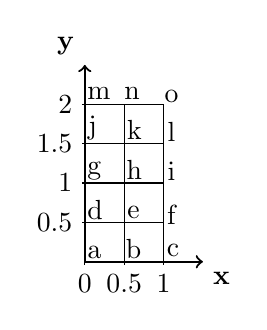
\begin{tikzpicture}

\draw[step=0.5cm,black] (0,0) grid (1,2);
\draw [thick,->](0,0) -- (1.5,0) node[anchor=north west] {\textbf{x}};
\draw [thick,->](0,0) -- (0,2.5) node[anchor=south east] {\textbf{y}};
\node at (0.12,0.12) {a};
\node at (0.62,0.165) {b};
\node at (1.12,0.14) {c};
\node at (0.13,0.66) {d};
\node at (0.62,0.62) {e};
\node at (1.1,0.6) {f};
\node at (0.12,1.15) {g};
\node at (0.63,1.17) {h};
\node at (1.1,1.15) {i};
\node at (0.1,1.7) {j};
\node at (0.63,1.68) {k};
\node at (1.1,1.65) {l};
\node at (0.18,2.14) {m};
\node at (0.6,2.14) {n};
\node at (1.1,2.1) {o};

\foreach \x in {0,0.5,1}
   \draw (\x cm,1pt) -- (\x cm,-1pt) node[anchor=north] {$\x$};
\foreach \y in {0.5,1,1.5,2}
    \draw (1pt,\y cm) -- (-1pt,\y cm) node[anchor=east] {$\y$};
\end{tikzpicture}
\end{center}

dengan penjabaran \(u(i,j)\) sebagai berikut.
\begin{center}
\begin{tabular}{c c c}
    \(u(1,5)=m\) & \(u(2,5)=n\) & \(u(3,5)=o\) \\
    %\hline
    \(u(1,4)=j\) & \(u(2,4)=k\) & \(u(3,4)=l\) \\
    %\hline
    \(u(1,3)=g\) & \(u(2,3)=h\) & \(u(3,3)=i\) \\
    %\hline
    \(u(1,2)=d\) & \(u(2,2)=e\) & \(u(3,2)=f\) \\
    %\hline
    \(u(1,1)=a\) & \(u(2,1)=b\) & \(u(3,1)=c\) \\
    %\hline
\end{tabular}
\end{center}

\subsection{Memasukkan Syarat Batas}
Setelah menandai perpotongan antar grid dengan node, maka node-node ini dapat dicari nilainya dengan mensubstitusikan ke dalam syarat batas.

\begin{center}
\begin{tabular}{c c|c} 
Grid & Node & Syarat batas \\ [0.5ex]
\hline  
 Bawah & a, b, c & \({u(x,0)=1}\) \\ [0.5ex]
 Atas & n & \(\frac{\partial \{u(x,2)\}}{\partial x}=0\) \\  [0.5ex]
 Kiri & d, g, j, m & \({u(0,y)=1}\) \\ [0.5ex]
 Kanan & f, i, l, o & \(\frac{\partial \{u(1,y)\}}{\partial y}=0\)\\ [0.5ex]
 Tengah & e, h, k & \( \frac{\partial^2 u}{\partial x^2}+{\frac{\partial^2 u}{\partial y^2}}=0\) \\

\end{tabular}
\end{center}
\bigskip

Untuk menyelesaikan persamaan diferensial parsial orde pertama pada syarat batas untuk grid atas dan grid kanan, kita dapat menggunakan pendekatan \textit{backward} sebagai berikut.
\[\frac{\partial u}{\partial x}= \frac {u(i,j)-u(i-1,j)}{\Delta x},\ dan\ \frac{\partial u}{\partial y}= \frac {u(i,j)-u(i,j-1)}{\Delta y}\]

\begin{itemize}
    \item \textbf{Grid atas}
        \subitem Dengan menggunakan persamaan diferensial parsial \textit{backward} orde kedua yang telah dituliskan di atas, maka dapat dijabarkan penyelesaiannya untuk syarat batas grid atas adalah sebagai berikut.
        \[\frac{\partial \{u(x,2)\}}{\partial x}=0\]
        \[\frac {u(i,j)-u(i-1,j)}{\Delta x}=0\]
        \[\frac {u(i,j)-u(i-1,j)}{\Delta x}=0\]
        \fbox{Misal, \(\frac {1}{\Delta x}=D\)}
        \[D(u(i,j))-D(u(i-1,j))=0\]
        \begin{equation}
        D(u(i,j))=D(u(i-1,j)) 
        \end{equation}
    \item \textbf{Grid kanan}
        \subitem Dengan cara yang sama seperti penyelesaian untuk grid atas, maka didapatkan penyelesaian syarat batas grid kanan adalah sebagai berikut.
        \[\frac{\partial \{u(1,y)\}}{\partial y}=0\]
        \[\frac {u(i,j)-u(i,j-1)}{\Delta y}=0\]
        \fbox{Misal, \(\frac {1}{\Delta y}=E\)}
        \[E(u(i,j))-E(u(i,j-1))=0\]
        \begin{equation}
        E(u(i,j))=E(u(i,j-1))\
        \end{equation}
    \item \textbf{Grid tengah}
        \subitem Untuk menyelesaikan persamaan diferensial orde kedua pada syarat batas grid tengah, kita dapat menggunakan persamaan (1) telah diselesaikan pada bagian sebelumnya.
        \begin{equation}
        A(u(i+1,j))+A (u(i-1,j))+ B(u(i,j+1))+B(u(i,j-1))+C(u(i,j))=0    \end{equation}
        %\[A(u(i+1,j))+A (u(i-1,j))+ B(u(i,j+1))+B(u(i,j-1))+C(u(i,j))=0\]
    \item \textbf{Grid bawah}
    \subitem Syarat batas untuk grid bawah adalah sebuah matriks identitas yang bernilai 1, ketika j=0 pada seluruh sumbu x.
    \begin{equation}
        u(x,0)=1
    \end{equation}
    \item \textbf{Grid kiri}
    \subitem Syarat batas untuk grid kiri adalah sebuah matriks identitas yang bernilai 1, ketika i=0 pada seluruh sumbu y.
    \begin{equation}
        u(0,y)=1
    \end{equation}
\end{itemize}

\subsection{Membuat Matriks \(15 \times 15\)}
Dari persamaan (2), (3), (4), (5), dan (6) yang telah dijabarkan  sebelumnya, maka kita dapat memvisualisasikan sebuah matriks berukuran \(15 \times 15 \) dengan ketentuan sebagai berikut.
\begin{enumerate}
    \item \textbf{Persamaan (2)} merupakan persamaan untuk batas atas yang dapat digunakan pada node n. Node n berada pada \(i=2\) dan \(j=5\).
    \item \textbf{Persamaan (3)} merupakan persamaan untuk batas kanan yang dapat digunakan pada node f, i, l dan o. Node f, i, l dan o berada pada \(i=3\) dan \(j=2,3,4,5\).
    \item \textbf{Persamaan (4)} merupakan persamaan untuk grid tengah yang dapat digunakan pada node e, h, dan k. Node e, h, dan k berada pada \(i=2\) dan \(j=2,3,4\).
    \item \textbf{Persamaan (5)} merupakan persamaan untuk batas bawah yang dapat digunakan pada node a, b, dan c. Node a, b, dan c berada pada \(i=1,2,3\) dan \(j=1\).
    \item \textbf{Persamaan (6)} merupakan persamaan untuk batas kiri yang dapat digunakan pada node d, g, j, dan m. Node d, g, j, dan m berada pada \(i=1\) dan \(j=2,3,4,5\).
\end{enumerate}

Dengan menggunakan ketentuan di atas, maka didapatkan visualisasi matriks \(Ax=B\) sebagai berikut.


\begin{displaymath}
%\noindent
\begin{+pmatrix}
\textbf{1} & 0 & 0 & 0 & 0 & 0 & 0 & 0 & 0 & 0 & 0 & 0 & 0 & 0 & 0 \\
0 & \textbf{1} & 0 & 0 & 0 & 0 & 0 & 0 & 0 & 0 & 0 & 0 & 0 & 0 & 0 \\
0 & 0 & \textbf{1} & 0 & 0 & 0 & 0 & 0 & 0 & 0 & 0 & 0 & 0 & 0 & 0 \\
0 & 0 & 0 & \textbf{1} & 0 & 0 & 0 & 0 & 0 & 0 & 0 & 0 & 0 & 0 & 0 \\
0 & \textbf{b} & 0 & \textbf{a} & \textbf{c} & \textbf{a} & 0 & \textbf{b} & 0 & 0 & 0 & 0 & 0 & 0 & 0 \\
0 & 0 & 0 & 0 & 0 & \textbf{e} & 0 & 0 & 0 & 0 & 0 & 0 & 0 & 0 & 0 \\
0 & 0 & 0 & 0 & 0 & 0 & \textbf{1} & 0 & 0 & 0 & 0 & 0 & 0 & 0 & 0 \\
0 & 0 & 0 & 0 & \textbf{b} & 0 & \textbf{a} & \textbf{c} & \textbf{a} & 0 & \textbf{b} & 0 & 0 & 0 & 0 \\
0 & 0 & 0 & 0 & 0 & 0 & 0 & 0 & \textbf{e} & 0 & 0 & 0 & 0 & 0 & 0 \\
0 & 0 & 0 & 0 & 0 & 0 & 0 & 0 & 0 & \textbf{1} & 0 & 0 & 0 & 0 & 0 \\
0 & 0 & 0 & 0 & 0 & 0 & 0 & \textbf{b} & 0 & \textbf{a} & \textbf{c} & \textbf{a} & 0 & \textbf{b} & 0 \\
0 & 0 & 0 & 0 & 0 & 0 & 0 & 0 & 0 & 0 & 0 & \textbf{e} & 0 & 0 & 0 \\
0 & 0 & 0 & 0 & 0 & 0 & 0 & 0 & 0 & 0 & 0 & 0 & \textbf{1} & 0 & 0 \\
0 & 0 & 0 & 0 & 0 & 0 & 0 & 0 & 0 & 0 & 0 & 0 & 0 & \textbf{d} & 0 \\
0 & 0 & 0 & 0 & 0 & 0 & 0 & 0 & 0 & 0 & 0 & 0 & 0 & 0 & \textbf{e}
\end{+pmatrix}
\begin{+pmatrix}
u(0,0)\\
u(1,0)\\
u(2,0)\\
u(0,1)\\
u(1,1)\\
u(2,1)\\
u(0,2)\\
u(1,2)\\
u(2,2)\\
u(0,3)\\
u(1,3)\\
u(2,3)\\
u(0,4)\\
u(1,4)\\
u(2,4)
\end{+pmatrix} =
\begin{+pmatrix}
1\\
1\\
1\\
1\\
0\\
e\\
1\\
0\\
e\\
1\\
0\\
e\\
1\\
d\\
e
\end{+pmatrix} \end{displaymath}

\bigskip
\subsection{Mencari Pola dan Membuat Kode}
Setelah mendapatkan \(Ax=B\) seperti di atas, maka dapat ditemukan pola pada matriks tersebut.

\subsubsection{Identifikasi Parameter Persoalan}
Untuk mengawali pembuatan code, alangkah lebih baiknya jika menuliskan inisiasi pada komponen-komponen yang akan ditampilkan pada code.
\begin{lstlisting}
    %inisiasi bidang persoalan
    x=1; y=2;
    
    %inisiasi parameter
    dx=1e-2; dy=2e-2; %delta x dan delta y (jarak antar titik pada sumbu x dan sumbu y)
    Nx=1+x/dx; Ny=1+y/dy; %banyaknya titik di x dan y
    xa=0:dx:(Nx-1)*dx; %panjangnya x pada kotak
    ya=0:dy:(Ny-1)*dy; %panjangnya y pada kotak
\end{lstlisting}

\subsubsection{Identifikasi Jenis Matriks}
Untuk menyelesaikan nilai \(x\), maka kita dapat mengidentifikasi komponen-komponen yang ada pada matriks A dan matriks B terlebih dahulu.
\begin{enumerate}
    \item Matriks A merupakan matriks persegi yang mempunyai dimensi baris dan kolom yang sama. Matriks A juga merupakan matriks diagonal dan matriks identitas. Namun untuk beberapa baris tertentu terdapat nilai yang tidak sama dengan nol untuk baris yang tidak tepat di diagonal, dan terdapat nilai yang tidak sama dengan satu untuk beberapa baris yang tepat di diagonal.
    \item Matriks B merupakan matriks kolom yang hanya mempunyai satu kolom dan beberapa baris
    
\end{enumerate}
Dari pola di atas, maka dapat dituliskan code untuk mengidentifikasi kedua matriks A dan matriks B.

\begin{lstlisting}
    A=eye(Nx*Ny); %matriks identitas
    B=zeros(Nx*Ny); %matriks zeros
\end{lstlisting}

\subsubsection{Membuat pola untuk setiap batas}
Berikut merupakan identifikasi awal sebelum membuat pola pada \textbf{matriks A}.
\begin{enumerate}
    \item Pada matriks A, terlihat pola bahwa matriks A merupakan matriks diagonal persegi namun pengecualian untuk baris 5, 8, dan 11. Ketiga baris ini memiliki nilai tidak sama dengan nol untuk kolom kolom di sekitarnya.
    \item Pada baris 6, 9, 12 dan 15, matriks diagonal A terisi dengan nilai \(e\). Sedangkan pada baris 14, matriks diagonal A terisi dengan nilai \(d\).
    \item Selain baris yang telah disebutkan pada nomor 1 dan 2, matriks diagonal A terisi nilai 1, yang berarti matriks identitas.
\end{enumerate}
Sedangkan berikut ini merupakan identifikasi sebelum membuat pola pada \textbf{matriks B}.
\begin{enumerate}
    \item Pada matriks B, terlihat pola untuk baris 5, 8, dan 11 memiliki nilai 0.
    \item Pada baris 6, 9, 12 dan 15, matriks B terisi dengan nilai \(e\). Sedangkan pada baris 14, matriks B terisi dengan nilai \(d\).
    \item Selain baris yang telah disebutkan pada nomor 1 dan 2, matriks B terisi nilai 1.
\end{enumerate}

\bigskip
Dari beberapa poin yang telah disebutkan di atas, maka dapat dicari beberapa komponen yang telah ada pada matriks A dan B, yaitu komponen bernilai 1, e, d, a, b, c. Dengan nilai a, b, c, d, dan e telah didefinisikan sebelumnya untuk penyelesaian persoalan dan syarat batas. Maka, kita dapat mendefinisikan nilai a, b, c, d, dan e terlebih dahulu pada matlab.
\begin{lstlisting}
    %permisalan persamaan
    a=1/dx^2; b=1/dy^2; c=-2*(a+b); 
    d=1/dx; e=1/dy; 
\end{lstlisting}

Setelahnya, kita dapat mencari pola untuk komponen bernilai 1, a, b, c, d, dan e.
\begin{itemize}
    \item \textbf{Komponen 1}
    \subitem Komponen 1 dapat dijumpai pada matriks diagonal A yang memenuhi syarat batas kiri dan syarat bawah saja. 
    \begin{enumerate}
        \item Syarat batas kiri berada pada \(i=1\) dan \(j=2,3,4,5\) atau \(j\) dapat dituliskan dengan \(j=1:Ny\) di program Matlab.
        \item Sedangkan syarat batas bawah berada pada \(i=1,2,3\) atau \(i\) dapat dituliskan dengan \(i=1:Nx\) pada program Matlab dan \(j=1\). 
        \item Dengan nilai matriks B pada syarat batas kiri dan bawah juga bernilai 1 pada baris-baris yang memenuhi. 
    \end{enumerate}
    
    Maka, code dapat dituliskan sebagai berikut dengan komponen k merupakan komponen yang berfungsi untuk menempatkan nilai matriks di baris dan kolom yang sesuai pada Matlab.
    \begin{lstlisting}
        %untuk batas bawah
        for ii=1:Nx
            jj=1; %batas bawah
            k=(jj-1)*Nx+ii;
            B(k,1)=1;
        end
        
        %untuk batas kiri
        for jj=1:Ny
            ii=1; %batas kiri
            k=(jj-1)*Nx+ii;
            B(k,1)=1; 
        end
    \end{lstlisting}

    \item \textbf{Komponen d}
    \subitem Komponen d dapat dijumpai pada matriks diagonal A yang memenuhi syarat batas atas saja dan dapat dijumpai pada matriks B dengan baris yang memenuhi syarat batas atas.
    \begin{enumerate}
        \item Syarat batas atas berada pada \(i=2\) atau \(i\) dapat dituliskan dengan \(i=2:Nx-1\) pada program Matlab. Dengan \(j=5\) atau \(j\) dapat dituliskan dengan \(j=Ny\) pada program Matlab. 
    \end{enumerate}
    Maka, code dapat dituliskan sebagai berikut dengan komponen k merupakan komponen yang berfungsi untuk menempatkan nilai matriks di baris dan kolom yang sesuai pada Matlab.
     \begin{lstlisting}
        %untuk batas atas
        for ii=2:Nx-1
            jj=Ny; %batas atas
            k=(jj-1)*Nx+ii;
            A(k,k)=d;
            B(k,1)=A(k,k-1);
        end
    \end{lstlisting}

    \item \textbf{Komponen e}
    \subitem Komponen e dapat dijumpai pada matriks diagonal A yang memenuhi syarat batas kanan saja dan dapat dijumpai pada matriks B dengan baris yang memenuhi syarat batas kanan.
    \begin{enumerate}
        \item Syarat batas kanan berada pada \(i=3\) atau \(i\) dapat dituliskan dengan \(i=Nx\) pada program Matlab. Dengan \(j=2,3,4,5\) atau \(j\) dapat dituliskan dengan \(j=2:Ny\) pada program Matlab. 
    \end{enumerate}
    Maka, code dapat dituliskan sebagai berikut dengan komponen k merupakan komponen yang berfungsi untuk menempatkan nilai matriks di baris dan kolom yang sesuai pada Matlab. 
     \begin{lstlisting}
        %untuk batas kanan
        for jj=2:Ny
            ii=Nx; %batas kanan
            k=(jj-1)*Nx+ii;
            A(k,k)=e;
            B(k,1)=A(k,k-Nx);
        end
    \end{lstlisting}
    
    \item \textbf{Komponen a, b, c}
    \subitem Ketiga komponen tersebut dapat dijumpai pada syarat batas tengah saja, yang dapat dijumpai pada baris ke 5, 8, dan 11 pada matriks A dan bernilai 0 pada baris yang sama di matriks B.
    \begin{enumerate}
        \item Syarat batas tengah berada pada \(i=2\) atau \(i\) dapat dituliskan dengan \(i=2:Nx-1\) pada program Matlab. Dengan \(j=2,3,4\) atau \(j\) dapat dituliskan dengan \(j=2:Ny-1\) pada program Matlab. 
        \item Nilai c berada pada koordinat diagonal matriks A.
        \item Nilai a berada pada satu kolom sebelum dan sesudah koordinat diagonal matriks A untuk baris yang sama.
        \item Nilai b berada pada tiga kolom sebelum dan sesudah koordinat diagonal matriks A untuk baris yang sama. Tiga kolom di sini sesuai dengan banyaknya node pada sumbu x pada permisalan awal pada bagian \textbf{2.1 Membuat Grid}, maka tiga kolom di sini dapat dimisalkan dengan \(Nx\).
    \end{enumerate}
    Maka, code dapat dituliskan sebagai berikut dengan komponen k merupakan komponen yang berfungsi untuk menempatkan nilai matriks di baris dan kolom yang sesuai pada Matlab. 
    \begin{lstlisting}
        %untuk titik-titik di tengah bidang
        for ii=2:Nx-1
            for jj=2:Ny-1
                k=(jj-1)*Nx+ii;
                A(k,k)=c;
                A(k,k-1)=a; A(k,k+1)=a;
                A(k,k-Nx)=b; A(k,k+Nx)=b;
                B(k,1)=0;
            end
        end
    \end{lstlisting}
\end{itemize}

\subsubsection{Membuat penyelesaian nilai x}
Untuk mendapatkan nilai x pada matriks berbentuk \(Ax=B\), maka dapat diselesaikan dengan cara sebagai berikut.
    \[Ax=B\]
\begin{equation}
    x=A^{-1} \times B
\end{equation}
Maka, untuk menyelesaikan persamaan di atas pada Matlab, kita dapat menuliskan code pada Matlab sebagai berikut. Dengan komponen k merupakan komponen yang berfungsi untuk menempatkan nilai matriks di baris dan kolom yang sesuai pada Matlab.
\begin{lstlisting}
    %mendapatkan nilai x pada persoalan
    solx=inv(A)*B; 
    for ii=1:Nx
        for jj=1:Ny
             k=(jj-1)*Nx+ii;
             sol(jj,ii)=solx(k);
        end
    end
\end{lstlisting}

\subsubsection{Memvisualisasikan hasil dengan colormap}
Untuk menampilkan hasil penyelesaian pada persamaan (7), maka dibuatlah sebuah grafik matriks berwarna yang menunjukkan nilai-nilai hasil dari penyelesaian matriks yang telah dibuat sebelumnya. Dibuatlah code sebagai berikut untuk menampilkan hasil nilai matriks x.
\begin{lstlisting}
    %plot visualisasi colormap pada matriks
    [X,Y]=meshgrid(xa,ya);
    surface (X,Y,sol);colormap("turbo");colorbar; 
    title('Solusi Permasalahan PDE', 'fontweight','bold')
    shading flat; axis ('equal')
    xlim([0 max(xa)]); ylim([0 max(ya)])
    xlabel('X', 'FontWeight','bold'); ylabel('Y', 'FontWeight','bold')
\end{lstlisting}

\newpage
\section{Source Code Lengkap}
\begin{lstlisting}
%%%%% Kelompok 23 Fiskom II nomor 3 %%%%%

clc;clear all;close all;
x=1; y=2; %bidang persoalan

%inisiasi parameter
dx=1e-2; dy=2e-2; %delta x dan delta y (jarak antar titik pada sumbu x dan sumbu y)
Nx=1+x/dx; Ny=1+y/dy; %banyaknya titik di x dan y
xa=0:dx:(Nx-1)*dx; %panjangnya x pada kotak
ya=0:dy:(Ny-1)*dy; %panjangnya y pada kotak

%permisalan persamaan
a=1/dx^2; b=1/dy^2; c=-2*(a+b); 
d=1/dx; e=1/dy; 

A=eye(Nx*Ny); %matriks identitas
B=zeros(Nx*Ny); %matriks zeros

%untuk batas bawah
for ii=1:Nx
    jj=1; %batas bawah
    k=(jj-1)*Nx+ii;
    B(k,1)=1;
end

%untuk batas kiri
for jj=1:Ny
    ii=1; %batas kiri
    k=(jj-1)*Nx+ii;
    B(k,1)=1; 
end

%untuk batas atas
for ii=2:Nx-1
    jj=Ny; %batas atas
    k=(jj-1)*Nx+ii;
    A(k,k)=d;
    B(k,1)=A(k,k-1);
end

%untuk batas kanan
for jj=2:Ny
    ii=Nx; %batas kanan
    k=(jj-1)*Nx+ii;
    A(k,k)=e;
    B(k,1)=A(k,k-Nx);
end

%untuk titik-titik di tengah bidang
for ii=2:Nx-1
    for jj=2:Ny-1
        k=(jj-1)*Nx+ii;
        A(k,k)=c;
        A(k,k-1)=a; A(k,k+1)=a;
        A(k,k-Nx)=b; A(k,k+Nx)=b;
        B(k,1)=0;
    end
end

%mendapatkan nilai persamaan 
solx=inv(A)*B; 
for ii=1:Nx
    for jj=1:Ny
        k=(jj-1)*Nx+ii;
        sol(jj,ii)=solx(k);
    end
end

%plot visualisasi colormap pada matriks
[X,Y]=meshgrid(xa,ya);
surface (X,Y,sol);colormap("turbo");colorbar; 
title('Solusi Permasalahan PDE', 'fontweight','bold')
shading flat; axis ('equal')
xlim([0 max(xa)]); ylim([0 max(ya)])
xlabel('X', 'FontWeight','bold'); ylabel('Y', 'FontWeight','bold')
\end{lstlisting}

\section{Hasil Running Source Code}
Berikut ini merupakan hasil \textit{run} dari \textit{source code} yang telah dituliskan sebelumnya.

\begin{figure} [h]
    \centering
    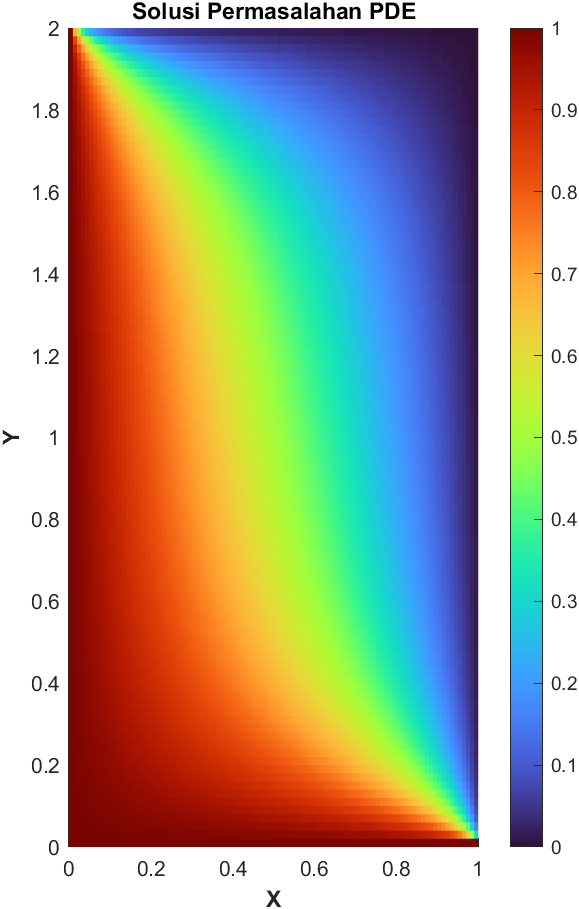
\includegraphics[width=6.8cm]{image/untitled101.png}
    \caption{Solusi Permasalahan PDE nomor 3 dalam 2D}
    \label{fig:2D}
\end{figure}

\begin{figure} [h]
    \centering
    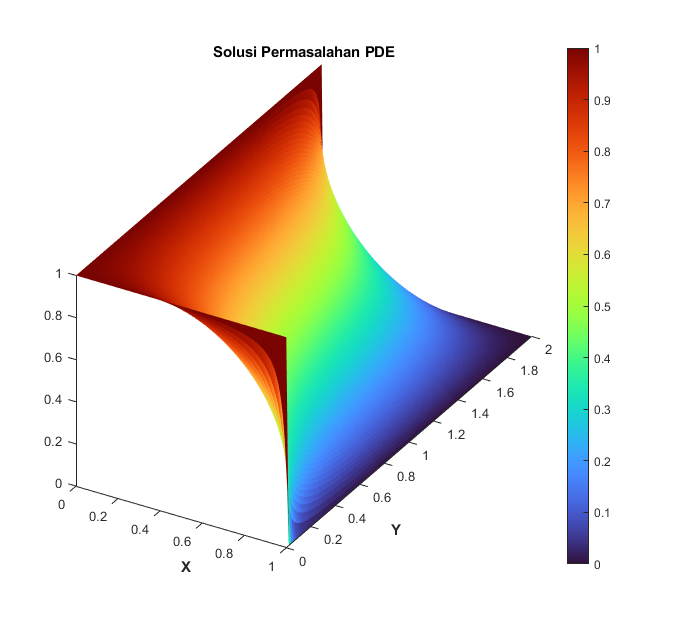
\includegraphics[width=\textwidth]{image/visualisasi3d2.png}
    \caption{Solusi Permasalahan PDE nomor 3 dalam 3D}
    \label{fig:3D}
\end{figure}
%%%

%\begin{itemize}
%    \item Batas bawah
%    \subitem \({u(x,0)=1},\ untuk\ {0\le x \le 1}\)
%    \item Batas atas
%    \subitem \( \frac{\partial \{u(x,2)\}}{\partial x}=0,\ untuk\ {0 \le x \le 1}\)
%    \item Batas kiri
%    \subitem \({u(0,y)=1},\ untuk\ {0 \le y \le 2}\)
%    \item Batas kanan
%    \subitem \( \frac{\partial \{u(1,y)\}}{\partial y}=0,\ untuk\ {0 \le y \le 2}\)
%\end{itemize}

\end{document}
